\chapter{Mathematical Background}

\section{Preliminaries}

We will first assemble the necessary mathematical background to understand the option pricing problem and build some foundations into the methods we will be using to solve it. The definitions and results are mostly standard, and can be found in textbooks such as \cite{karatzas2014brownian, karatzas1998methods} but we will cover them here for self-containment and to set up notation for the rest of the project. As a result, we will only cover the main concepts and not delve too deeply into the details, since our focus is more on the numerical methods and their applications in this project.

\subsection{Probabilistic Setup}

To begin, we require a formalisation of the underlying randomness in our model for the market, which will be done through probability spaces and filtrations. The pricing problem is inherently probabilistic, as we are uncertain about the future evolution of the underlying asset price, thus requiring a rigorous mathematical framework to model this uncertainty.

\begin{definition}[Probability space]
    A \textit{probability space} is a triple $(\Omega, \mathcal F, \mathbb P)$ where $\Omega$ is the sample space, $\mathcal F$ is a $\sigma$-algebra on $\Omega$, and $\mathbb P: \mathcal F \to [0, 1]$ is a probability measure such that $\mathbb P(\Omega) = 1$.
\end{definition}

The arrival of information through time in the market is modelled by a filtration.

\begin{definition}[Filtration, filtered probability space]
    A \textit{filtration} on the probability space $(\Omega, \mathcal F, \mathbb P)$ is a non-decreasing family $(\mathcal F_t)_{t \ge 0}$ of sub-$\sigma$-algebras of $\mathcal F$, that is to say, $\mathcal F_s \subseteq \mathcal F_t \subseteq \mathcal F$ for all $s \le t$. The quadruple $(\Omega, \mathcal F, \{\mathcal F_t\}_{t \ge 0}, \mathbb P)$ is called a \textit{filtered probability space}.
\end{definition}

We will also define a Martingale, which formalises the idea that future expectations of a process are equal to the current value, which is a key concept in the risk-neutral pricing framework.

\begin{definition}[Martingale]
    A process $M = (M_t)_{t \ge 0}$ is a \textit{martingale} with respect to the filtration $\{\mathcal F_t\}$ and the probability measure $\mathbb P$ if $\mathbb E[M_t \mid \mathcal F_s] = M_s$ for all $0 \le s \le t$.
\end{definition}

The Markov assumption is also commonly made in financial modelling and will also be made in our project, which states that the future evolution of the process only depends on the current state and not on the past history.

\begin{definition}[Markov process]
    A process $X = (X_t)_{t \ge 0}$ is a \textit{Markov process} with respect to the filtration $\{\mathcal F_t\}$ if
    \begin{equation}
        \mathbb E[f(X_t) \mid \mathcal F_s] = \mathbb E[f(X_t) \mid X_s]
    \end{equation}
    for all $0 \le s \le t$ and all bounded measurable functions $f$.
\label{def:markov_process}
\end{definition}

\subsection{Stochastic processes}

The market in practice is not deterministic, so we will mathematically construct our model with stochastic processes.

\begin{definition}[Stochastic process]
    A \textit{stochastic process} is a family of random variables $\{X_t : t \ge 0\}$ defined on a probability space $(\Omega, \mathcal F, \mathbb P)$.
\end{definition}

More specifically, we will use Brownian motion to model the underlying asset price dynamics, which is a continuous-time stochastic process with continuous paths and stationary independent increments.

\begin{definition}[Brownian motion]
    A real-valued process $W = (W_t)_{t \ge 0}$ on the probability space ($\Omega, \mathcal F, \mathbb P$) is a \textit{Brownian motion} if it satisfies the following properties:
    \begin{itemize}
        \item $W_0 = 0$ almost surely
        \item The increment $W_t - W_s$ is normally distributed with mean $0$ and variance $t-s$ for all $0 \le s < t$
        \item The increments $W_{t_1} - W_{t_0}, \dots, W_{t_n} - W_{t_{n-1}}$ are independent for all $0 \le t_0 < t_1 < \dots < t_n$
        \item The sample paths $t \mapsto W_t(\omega)$ are continuous
    \end{itemize}
\end{definition}

The existence of this process is established by Wiener \cite{wiener1923differential} and is very powerful in modelling the randomness in the financial market.

\subsection{Risk-neutral pricing}

We will now formalise the financial market and establish the principle of arbitrage-free valuation that will underpin our option pricing problem.

In our model, the market involves a fixed horizon $T > 0$ (our expiry) and a filtered probability space $(\Omega, \mathcal F, \{\mathcal F_t\}_{t \in [0, T]}, \mathbb P)$ where $\{\mathcal F_t\}$ is the filtration generated by the underlying Brownian motion. The market consists of a risk-free asset $B_t$ that is deterministic and follows the evolution
\begin{equation}
    B_t = \exp\left(\int_0^t r(s) \,\mathrm ds\right)
\end{equation}
and one or more risky assets $S_t$ that follows an Itô process.

It is important that the market is arbitrage-free, which means that there does not exist any trading strategy that can generate a positive profit with zero initial investment and zero risk. To formalise this, we first define a trading strategy $\phi$ that is self-financing, which means that that any change in the value of the portfolio is only due to changes in the assets held, without any external cash flow.

\begin{definition}[Self-financing trading strategy]
    A \textit{self-financing trading strategy} $\phi$ is a predictable process such that the value of the portfolio $V_t = \phi_t^B B_t + \phi_t^S S_t$ satisfies
    \begin{equation}
        \mathrm d V_t = \phi_t^B \mathrm d B_t + \phi_t^S \mathrm d S_t
    \end{equation}
\end{definition}

\begin{definition}[Arbitrage]
    An \textit{arbitrage} is some trading strategy $\phi$ such that $V_0 = 0$, $V_T \ge 0$ almost surely and $\mathbb P(V_T > 0) > 0$.
\end{definition}

By the fundamental theorem of asset pricing, the market is arbitrage-free if and only if there exists a measure $\mathbb Q$ such that $\mathbb Q$ is equivalent to $\mathbb P$ (they have the same null sets) and the discounted price process $\tilde S_t = \frac{S_t}{B_t}$ is a martingale under $\mathbb Q$.

Given that the market is arbitrage-free, we can price any derivative with payoff $g(\cdot)$ at time $t$ by taking the discounted expectation of the payoff under the risk-neutral measure $\mathbb Q$, giving us the risk-neutral pricing formula for European derivative with maturity $T$:

\begin{equation}
    v(t, S) = B_t \mathbb E^\mathbb Q \left[\frac{g(S_T)}{B_T} \mid \mathcal F_t\right]
\end{equation}

For this project, we will deal with constant interest rates, so the bond price process reduces to $B_t = e^{rt}$ where $r$ is the constant risk-free rate. Additionally, we will also assume the Markov property (\ref{def:markov_process}). The arbitrage-free price of the European derivative will therefore be given by

\begin{equation}
    v(t, S_t) = e^{-r(T-t)} \mathbb E^\mathbb Q \left[g(S_T) \mid S_t\right]
\end{equation}

\subsection{Optimal stopping problem}

The American option gives the holder the right to exercise the option at any time before maturity, which thus gives us the interpretation of the option price as the solution to an optimal stopping problem.

\begin{definition}[Stopping time]
    A random variable $\tau : \Omega \to [0, \infty]$ is a \textit{stopping time} if $\{\tau \le t\} \in \mathcal F_t$ for all $t \ge 0$.
\end{definition}

The price of the American option can thus be expressed as the $\mathbb Q$-expectation of the discounted payoff at the optimal stopping time $\tau^\star$ that maximises the expected payoff, giving the optimal stopping problem

\begin{equation}
    v(t, S_t) = \sup_{\tau \in [t, T]} \mathbb E^\mathbb Q \left[e^{-r(\tau - t)} g(S_\tau) \mid S_t \right]
\end{equation}

\subsection{Continuation region and free boundary}

The optimal stopping problem for the American put option gives rise to the problem of finding the free boundary, which is the boundary separating the exercise region and the continuation region. As before, the value of the American put with strike $K$ and maturity $T$ on a risky asset $S$ is given by the optimal stopping problem

\begin{equation}
    v(0, S) = \sup_{\tau \in [0, T]} \mathbb E\big[e^{-r\tau}(K - S_\tau)^+\big]
\end{equation}

which is achieved by an optimal stopping time $\tau^\star$ taking the form

\begin{equation}
    \tau^\star = \inf\{t \ge 0 : S(t) \le b^\star(t)\}
\end{equation}

for some optimal exercise boundary $b^\star(t)$ \cite{glasserman2004monte}. This is illustrated in Figure \ref{fig:free_boundary}, where we simulate one realisation of the asset price assuming a geometric Brownian motion and plot it against the exercise boundary, which is found using binary search on the binomial tree solution, where we have

\begin{equation}b^\star(t) = \inf\{S : c(t, S) > g(S)\}\end{equation}

where $c(t, S)$ is the continuation value of the option with payoff $g(S)$.

\begin{figure}[h!]
    \centering
    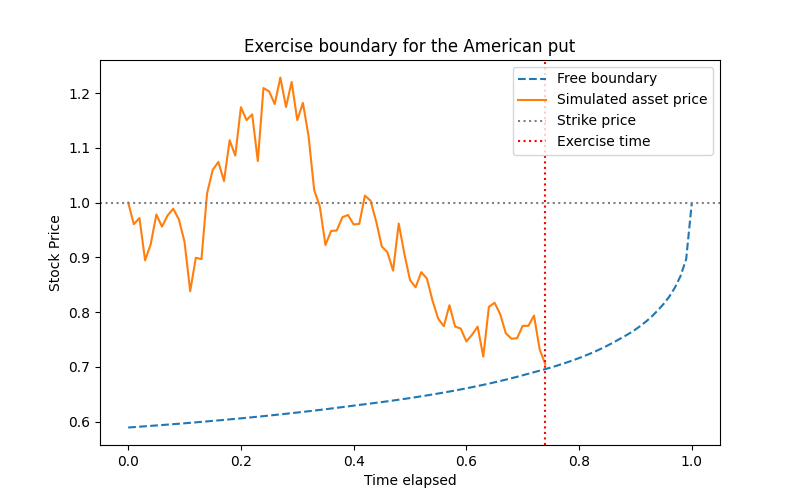
\includegraphics[width=0.8\textwidth]{../plots/mathematical_background/free_boundary.png}
    \caption{Exercise boundary for the American put}
    \label{fig:free_boundary}
\end{figure}

This formulation describes a hard classification problem, where we classify points in the time-stock price space binarily to be either in the continuation region or the exercise region. However, our numerical solutions to the pricing problem are not exact and there is some level of error in the solution that comes from the Monte Carlo simulations upon the space, the numerical differentiation used in training and the early stopping in the training process. Therefore, it would be more intuitive to perform a soft classification instead, where we assign probabilities to points in the time-stock price space to be in the continuation region or the exercise region, which would give us a more intuitive visualisation of the free boundary and how it evolves over time. We will do this by extending hard classification: that is to say, the continuation region $A$ is

\begin{equation}
    A = \{(t, S) : c(t, S) > g(S)\} \cup \{(t, S) : g(S) = 0\}
\end{equation}

where intuitively, the first set is those where the continuation value is greater than the early exercise value, and the second set is those where the payoff is zero, which are at-the-money and out-of-the-money options that are worthless under immediate exercise.

We will consider two methods to extend the definition of the continuation region to a soft classification. The first one is to use a sigmoid function $s: \mathbb R \to (0, 1)$ defined as

\begin{equation}
    s(x) = \frac{1}{1 + e^{-x}}
\end{equation}

to smoothly transition the continuation probability from $0$ to $1$ as the value function transitions from being below the payoff to being above the payoff. As the sigmoid function is the CDF of the logistic distribution, we can interpret this as modelling the noise in the value function as a logistic distribution. The effect of the noise can be controlled by introducing the softness parameter $\tau > 0$, and our continuation probability function can be defined on the relative difference from the payoff as

\begin{equation}
    P_\text{cont}(d) = s\left(\frac d \tau\right),
    \qquad d := \frac{c(t, S) - g(S)}{g(S)}
\end{equation}

To tune the softness parameter, we can define a threshold $I \in (0.5, 1)$ such that we want the continuation probability to be $I$ at some relative difference $\epsilon > 0$, i.e. $P_\text{cont}(\epsilon) = I$, which we could solve with some simple algebraic manipulation to get
\begin{equation}
    \tau = \frac{\epsilon}{\ln\left(\frac{I}{1 - I}\right)}
\end{equation}

The second method is to assume Gaussianity of the noise in our estimate $\hat c$ of the continuation value, or in other words
\begin{equation}
    \hat c(t, S) = c(t, S) + \epsilon, \qquad \epsilon \sim \mathcal N(0, \tilde \sigma^2)
\end{equation}
where $c$ is the true (latent) continuation value and $\tilde \sigma$ is the standard deviation of the noise, which is unknown. We can then perform $n$ simulations of the solution to get $\hat c_1, \dots, \hat c_n$ and use the sample mean $\bar c$ as our unbiased estimate of the continuation value function, and the sample standard deviation $\hat \sigma$ as our estimate. Then $\bar c$ is distributed according to a $t$-distribution with $n-1$ degrees of freedom, and we can compute the continuation probability as
\begin{equation}
    P_\text{cont}(t, S) = \mathbb P_{t_{n-1}}\left( \frac{\bar c(t, S) - g(S)}{\hat \sigma(t, S) / \sqrt n} > 0 \right)
\end{equation}

The caveat with this method is that it requires multiple simulations of the solution, which becomes infeasible for more complex models and higher dimensions, but it gives us a more statistically grounded way to compute the continuation probability.

All that is left is to find a method to obtain the continuation value function, as it is generally latent and not directly observable, given that we predict the American option price that already takes the maximum of the continuation value and the payoff. However, we can use

\begin{equation}
    c(t, S) = \mathbb E\left[e^{-rh} f(t+h, S_{t+h})\mid S_t = S\right]
\end{equation}

where $h > 0$ is a small time step and $f$ is the American option price function. We can estimate this expectation by simulating the asset price $S_{t+h}$ at time $t+h$ given $S_t=S$ and evaluating the option price function at the point, then taking the average across all simulations.

\section{State Space Discretisation}

\subsection{Background}

Recall that the option value function $v(t, x)$ is the solution to the optimal stopping problem
\begin{equation}
    v(t, S) = \sup_{\tau \in [t, T]} \mathbb E\left[ e^{-r(\tau - t)} g(S_\tau) \mid S_t = S \right]
\end{equation}

There does not exist a closed-form solution for this problem in general, and thus we have to resort to numerical methods. We first consider methods that discretise the continuous time into a finite grid $\{t_i\}_{i=1}^N$ where we have
\begin{equation}
    0 = t_0 < t_1 < \dots < t_N = T
\end{equation}
which we can use to index the underlying state variable $S_{t_i}$ at time $t_i$. Note that the state variable $S_{t_i}$ could depend on multiple variables, such as in the Heston model, where we have a stochastic variance term encoded in the asset price. The goal is to compute the arbitrage-free price $v(0, S_0)$ at time $t=0$ given the initial state $S_0$. As we know the solution must satisfy the terminal condition $v(T, S) = g(S)$ for all $S$, we can use backward induction to compute the option value at each time step. This gives rise to the class of numerical methods known as tree methods.

\subsection{Tree Methods}

In a tree model, we discretise the time-state space into a finite grid, where the state variable $S_{t_i}$ can take a finite number of values at each time step given the previous one. We will particularly explore binomial trees in this project, where each state can evolve to one of two possible states at the next time step. Formally, suppose at time $t_n$ we have the state $S_{t_n} \in \{S_n^1, \dots, S_n^{M_n}\}$ where $M_n$ is the number of possible states at time $t_n$. Then at time $t_{n+1}$, each state $S_n^i$ can evolve to the state $S_{n+1}^j$ with transition probability
\begin{equation}
    p_{ij}^{(n)} = \mathbb P(S_{n+1} = S_{n+1}^j \mid S_n = S_n^i)
\end{equation}
This is a discrete-time Markov chain, and to identify the transition probabilities, we can use the risk-neutral condition which states that the discounted price process must be a martingale under the risk-neutral measure. This gives us the condition
\begin{equation}
    \sum_{j=1}^{M_{n+1}} p_{ij}^{(n)} S_{n+1}^j = e^{r\Delta t} S_n^i
\end{equation}
where $\Delta t = t_{n+1} - t_n$ and $r$ is the risk-free rate.

With these transition probabilities, we can compute the option value at time $t_n$ given the option value at time $t_{n+1}$ by using backwards induction, which gives us the recursive relation
\begin{equation}
    v(t_n, S_n^i) = \max\left( g(S_n^i), e^{-r\Delta t} \sum_{j=1}^{M_{n+1}} p_{ij}^{(n)} v(t_{n+1}, S_{n+1}^j) \right)
\end{equation}

where we take the maximum of the payoff and the discounted expected future price to account for early exercise for the American option. This maximum operator can easily be lifted for all time steps for European options, or only imposed on certain time steps for Bermudan options, leaving the tree method a very flexible method. This backwards induction is applied iteratively starting from the terminal condition at time $t_N = T$ to compute the option value at time $t_0 = 0$.

An issue with tree methods is that the number of states $M_n$ can grow exponentially with the number of time steps $N$, leading to a very computationally expensive algorithm. To mitigate this, we can use recombining trees where the states at each time step are designed to recombine with each other, so that the number of states $M_n$ grows linearly. Another issue is that, while flexible, the tree method can be difficult to implement for more complex models where the state depends on multiple variables or if we wish to extend it to options operating on multiple assets, but its reliability and interpretability make it a good benchmark for simpler models.

\section{Physics-Informed Neural Networks}
\label{sec:pinns}

\subsection{Motivation}
Our option pricing problem can alternatively be formulated as a variational inequality which takes the form of a partial differential equation that is independent from the payoff $g(\cdot)$. These PDEs can be of high dimension, and are thus difficult to solve using traditional numerical methods due to the curse of dimensionality. Traditional methods such as finite difference methods require discretisation of the domain and the number of grid points (and hence algorithm complexity) scales exponentially $\mathcal O(N^d)$ with the dimension $d$ of the problem.

We can attempt a neural network solution to the PDEs, as neural networks are known to be universal approximators. That is, suppose we have the class of functions $\mathcal F$ over a compact set $S$ that can be represented by a neural network with a given architecture, with a continuous target function $f^\star$ that we would like to approximate. Then for any target accuracy $\epsilon > 0$, there exists a function $f \in \mathcal F$ such that
\begin{equation}
    \sup_{x \in S} |f(x) - f^\star(x)| \le \epsilon
\end{equation}
If we have a squashing activation function $\Psi(\cdot)$ that is non-decreasing and satisfies the limits
\begin{equation}
    \Psi(-\infty) = 0, \quad \Psi(\infty) = 1
\end{equation}
then the class of functions $\mathcal F$ that can be represented by a neural network with one hidden layer and activation function $\Psi$ is dense in the space of continuous functions on $S$ and thus is a universal approximator \cite{hornik1989multilayer}.

Since the option price function is continuous in the time-asset price domain, we can use a neural network to find an approximation. This is favourable because the time complexity scales with the number of parameters, which is not exponential. To do this, we will use the framework of physics-informed neural networks (PINNs) to solve the PDEs, which have been shown to be effective for solving high-dimensional PDEs \cite{raissi2019physics}, by avoiding mesh construction and leveraging the interpolation capability of neural networks \cite{hu2024tackling}. The loss function of the neural network is designed to penalise deviations from the PDE as well as deviations from the boundary conditions. By training the neural network to minimise this loss function, we can obtain an approximation to the solution of the PDE. This method has been applied to option pricing problems in the literature, such as in \cite{dhiman2023physics} for the Black-Scholes model, but we will look to apply it to more complex models such as the Heston model as well as to options on multiple assets. 

\subsection{Methodology}
We first provide a general setup for PINNs, before modifying it to tailor our specific problem of option pricing. Formally, suppose we have an unknown latent solution $u(t, x)$ which is governed by a PDE of the form
\begin{equation}
    \frac{\partial u}{\partial t} + \mathcal L[u] = 0, \qquad t \in [0, T], x \in \Omega
\end{equation}
where $\mathcal L$ is a (not necessarily linear) differential operator. Suppose additionally that this PDE is subject to the boundary conditions
\begin{align}
    u(0, x) &= g(x), \qquad x \in \Omega \\
    \mathcal B[u] &= 0, \qquad t \in [0, T], x \in \partial \Omega
\end{align}
where $\mathcal B$ is a boundary operator. Then the unknown solution $u$ can be approximated by a deep neural network $f_\theta(t, x)$ where $\theta$ are the parameters of the neural network, trained by minimising a loss function composed of deviations from the PDE residual, boundary conditions and initial conditions \cite{wang2023expert}:
\begin{equation}
    L(\theta) = \lambda_{r}L_{r}(\theta) + \lambda_{bc}L_{bc}(\theta) + \lambda_{ic}L_{ic}(\theta)
\end{equation}
where the loss components are mathematically defined as
\begin{align}
    L_{r}(\theta) &= \frac{1}{N_r}\sum_{i=1}^{N_r} \left| \mathcal R_\theta(t_r^i, x_r^i) \right|^2 \\
    L_{bc}(\theta) &= \frac{1}{N_{bc}} \sum_{i=1}^{N_{bc}} \left| \mathcal B[f_\theta](t_{bc}^i, x_{bc}^i) \right|^2 \\
    L_{ic}(\theta) &= \frac{1}{N_{ic}} \sum_{i=1}^{N_{ic}} \left| f_\theta(0, x_{ic}^i) - g(x_{ic}^i) \right|^2
\end{align}

where the PDE residual $\mathcal R_\theta$ is defined as
\begin{equation}
    \mathcal R_\theta(t, x) = \frac{\partial f_\theta}{\partial t}(t, x) + \mathcal L[f_\theta](t, x)
\label{eq:pde_residual}
\end{equation}
We additionally use the sampled points $\{x_{ic}^i\}_{i=1}^{N_{ic}}$ from the initial condition domain, $\{(t_{bc}^i, x_{bc}^i)\}_{i=1}^{N_{bc}}$ from the boundary condition domain and $\{(t_r^i, x_r^i)\}_{i=1}^{N_r}$ from the PDE domain, sampled uniformly in their respective domains at each iteration of the gradient descent algorithm.

There are different methods to choose the loss weights $\lambda_r, \lambda_{bc}, \lambda_{ic}$, such as using fixed weights or using adaptive weights that change during training. For simplicity, we will use fixed weights in the project.

For our specific problem of option pricing, we can modify the above setup to fit our variational inequality formulation. The PDE to solve is dependent on the model for the asset dynamics, and the boundary conditions are given by the payoff function of the option. In general, we will have to solve a problem of the form
\begin{align}
    \min\left\{ -\frac{\partial u}{\partial t} + \mathcal L[u], u - g \right\} &= 0, \qquad t \in [0, T], x \in \Omega \label{eq:pinn_pde}\\
    u(T, x) &= g(x), \qquad x \in \Omega \label{eq:pinn_terminal}\\
    \mathcal B_k[u] &= 0 \qquad t \in [0, T], x \in \partial \Omega, k=1, \dots, K \label{eq:pinn_boundary}
\end{align}
where $k$ indexes the $K$ different boundary conditions. This is very similar to the general setup for PINNs, except that we have a variational inequality instead of a PDE, and we have a terminal condition instead of an initial condition. However, we can still use the framework by noting we can make the substitution $t \mapsto T-t$ to un-negate the negative partial derivative in the PDE term and to convert the terminal condition to an initial condition. The variational inequality can be handled by modifying the PDE residual loss (\ref{eq:pde_residual}) to
\begin{equation}
    \mathcal R_\theta(t, x) = \min\left\{ \frac{\partial f_\theta}{\partial t}(t, x) + \mathcal L[f_\theta](t, x), f_\theta(t, x) - g(x) \right\}
\end{equation}

\section{Sobolev Deep Neural Networks}

We can explore a different method to price American puts with neural networks, where this time we work with fractional Sobolev norms to construct our loss function. This is motivated by the fact that we would be able to guarantee that our neural network converges to the true solution provided that its loss converges instead of just pointwise convergence. Additionally, the loss function components no longer depend on the payoff and is applicable for all situations, a desirable property for a general method.

\subsection{Preliminaries}

The theory of Sobolev spaces are rich and we will not attempt to cover all the details to not divert the attention from the main focus of the project, but we will cover the necessary background to understand the method.

\subsubsection{Sobolev Spaces}

We first introduce the concept of Sobolev spaces. To bein, we consider those of integer order, defined over an arbitrary domain $\Omega \subset \mathbb R^n$, but we will generalise to fractional orders later. These are vector subspaces of various Lebesgue spaces $L^p(\Omega)$, which is the class of all measurable functions $u$ for which
\begin{equation}
    \int_\Omega |u(x)|^p \,\mathrm dx < \infty
\end{equation}

The Sobolev norms are functionals $\|\cdot\|_{m, p}$ where $m \in \mathbb N_+$ and $1 \le p \le \infty$, defined as follows:
\begin{align}
    \|u\|_{m, p} &= \left(\sum_{0 \le |\alpha|\le m} \|D^\alpha u\|^p_p\right)^{1/p} \qquad  1 \le p < \infty \\
    \|u\|_{m, \infty} &= \max_{0 \le |\alpha| \le m }\|D^\alpha u\|_\infty
\end{align}
where $\|\cdot\|_p$ is the norm in $L^p(\Omega)$. The Sobolev spaces are consequently those on which $\|\cdot \|_{m, p}$ is a norm \cite{adams2003sobolev}:
\begin{itemize}
    \item $H^{m, p}(\Omega) \equiv \text{the completion of } \{u \in C^m (\Omega) : \|u\|_{m, p} < \infty\}$ with respect to the norm $\|\cdot \|_{m, p}$
    \item $W^{m, p}(\Omega) \equiv \{u \in L^p(\Omega) : D^\alpha u \in L^p(\Omega) \text{ for } 0 \le |\alpha| \le m \}$ where $D^\alpha u$ is the weak partial derivative
    \item $W_0^{m, p}(\Omega) \equiv \text{the closure of }C^\infty_0 \text{ in the space } W^{m, p}(\Omega)$
\end{itemize}

It can be shown by Theorem 3.17 of \cite{adams2003sobolev} that for $1 \le p < \infty$ we have
\begin{equation}
    H^{m, p}(\Omega) = W^{m, p}(\Omega)
\end{equation}
so for the rest of this section, we will use the space $H^{m, p}(\Omega)$.

\subsubsection{Fractional Sobolev Spaces}

Suppose we have a general, possibly nonsmooth, open set $\Omega \subset \mathbb R^n$. For any real $s > 0$ and for any $p \in [1, \infty)$, we aim to define the fractional Sobolev spaces $W^{s, p}(\Omega)$.

To construct this, let's first fix the fractional exponent $s \in (0, 1)$. Then for any $p \in [1, +\infty)$ we define $W^{s, p}(\Omega)$ as \cite{di2012hitchhikers}:
\begin{equation}
    W^{s, p}(\Omega) := \left\{u \in L^p(\Omega) : \frac{|u(x) - u(y)|}{|x-y|^{\frac np + s}} \in L^p(\Omega \times \Omega)\right\}
\end{equation}
which can be interpreted as an intermediary Banach space between $L^p(\Omega)$ and $W^{1, p}(\Omega)$ endowed with the norm
\begin{equation}
    \|u\|_{W^{s, p}(\Omega)} := \left(\int_\Omega |u|^p \,\mathrm dx + \int_\Omega \int_\Omega \frac{|u(x)-u(y)|^p}{|x-y|^{n+sp}}\,\mathrm dx \mathrm dy\right)^{\frac 1p}
\end{equation}
where we have used the \textit{Gagliardo seminorm} of $u$:
\begin{equation}
    [u]_{W^{s, p}(\Omega)} := \left( \int_\Omega \int_\Omega \frac{|u(x)-u(y)|^p}{|x-y|^{n+sp}}\,\mathrm dx \mathrm dy\right)^{\frac 1p}
\end{equation}

\subsection{Model}
Suppose we would like to price an option on $k$ assets $\bm S = (S^1, \dots, S^k)$. Similar to before, these assets have theoretically unbounded prices, so we need to truncate it a minimum and maximum price in our model. Thus the domain of the target function can be chosen to be

\begin{equation}
    \Omega = (S_\text{min}^1, S_\text{max}^1) \times \cdots \times (S_\text{min}^k, S_\text{max}^k)
\end{equation}

In our study we will make the simplification that $S_\text{min}^i = S_\text{min}^j$ and $S_\text{max}^i = S_\text{max}^j$ for all $i \ne j$, which we can call $a$ and $b$ respectively. Our spaces would consequently have the definitions

\begin{equation}
    \Omega = (a, b)^n \qquad \Omega_T = (0, T) \times \Omega \qquad \Sigma = (0, T) \times \partial \Omega
\end{equation}

where $\partial \Omega =: \Gamma$ is the boundary of $\Omega$, a hyper-rectangle. We will use the representation

\begin{equation}
    \Gamma = \bigcup_{i=1}^n \big(\{x \in [a, b]^n : x_i = a\} \cup \{x \in [a, b]^n : x_i = b\} \big)
\end{equation}
which is not the simplest, but it is useful as it is decomposed into faces, which is useful when we would like to use the norm derivative later. Note that in the one-dimensional case, this reduces simply to the points $\{a, b\}$.

\subsection{Loss function}
Our loss function would be a weighted sum of four loss components $\sum_{i=1}^4 \lambda_iJ_i$, each of which ensures regulation of a specific aspect of our function.

\begin{enumerate}
    \item The variational loss, which is as before, controlling the accuracy of our function in the interior of our domain:
    \begin{equation}
        J_1 = \|\min \{\mathcal G[f], f-g\}\|^2_{L^2(\Omega_T), \mu_1}
    \end{equation}
    \item The energy loss: before we were only controlling the L2 norm of the payoff, but we require the option value to equal the payoff as a function and not just pointwise. Thus we need to incorporate the gradient into the loss so that the spatial slope of the payoff is respected.
    \begin{equation}
        J_2 = \|f(0, \cdot) - g(\cdot) \|^2_{H^1(\Omega), \mu_2}
    \end{equation}
    where we have the norm defined as
    \begin{equation}
        \|d\|^2_{H^1(\Omega), \mu_2} = \|d\|^2_{L^2(\Omega)} + \|\nabla d\|^2_{L^2(\Omega)}
    \end{equation}
    and the derivative
    \begin{equation}\nabla d = \big(\partial_{x_1}d, \dots, \partial_{x_k}d\big)\end{equation}
    \item J3 (need to explain intuitively)
    \begin{equation}
        J_3 =\|f(t, x) - g( x)\|^2_{H^{\frac 34, \frac 32}(\Sigma), \mu_3}
    \end{equation}
    where
    \begin{align}
        \|d\|^2_{H^{\frac 34, \frac 32}(\Sigma)} = \|d\|^2_{H^{0,1}(\Sigma)} &+ \int_0^T\int_0^T\frac{\|d(t_1, \cdot) - d(t_2, \cdot)\|^2_{L^2(\Gamma)}}{|t_1-t_2|^{2.5}}\,\mathrm dt_1\,\mathrm dt_2 \\ &+ \int_0^T\int_\Gamma\int_\Gamma \frac{|d(t, x) - d(t, y)|^2}{\|x-y\|^{2}}\,\mathrm d\sigma(x)\mathrm d\sigma(y) \mathrm dt
    \end{align}
    The time exponent $2.5$ is equal to $2p+1$ where $p$ is the decimal part of the time fractional exponent, and the space exponent $2$ is equal to $2\theta + k - 1$ where $\theta$ is the decimal part of the space fractional exponent, and $k$ the dimension. Note that here $\mathrm d \sigma(x)$ and $\mathrm d \sigma(y)$ indicate the surface measures on $\Gamma$, but in practice we can treat these as $\mathrm dx$ and $\mathrm dy$.
    \item J4 (need to explain intuitively):
    \begin{equation}
        J_4 =\left\|\nabla (f-g) \cdot v\right\|^2_{H^{\frac 14, \frac 12}(\Sigma), \mu_4}
    \end{equation}
    where the norm derivative is $\nabla(f-g)\cdot \nu = \partial_{x_{i^\star}}(f-g)$ given that $x_{i^\star} \in \{a, b\}$ and $x_{i} \in (a, b)$ for $i \ne i^\star$. Rigorously, we require the sign but in practice this is not necessary, as we will square in the end. The fractional norm is thus written
    \begin{align}
        \|d\|^2_{H^{\frac 14, \frac 12}(\Sigma)} = \|d\|^2_{L^2(\Sigma)} &+ \int_0^T\int_0^T \frac{\|d(t_1, \cdot) - d(t_2, \cdot)\|^2_{L^2(\Gamma)}}{|t_1-t_2|^{1.5}}\,\mathrm dt_1\mathrm dt_2 \\ &+ \int_{0}^T\int_\Gamma\int_\Gamma \frac{|d(t, x) - d(t, y)|^2}{\|x-y\|^2}\,\mathrm d\sigma(x)\mathrm d(y)\mathrm dt
    \end{align}
    because $H^{0, 0} = L^2$.
\end{enumerate}

In practice, we will compute a Monte Carlo estimate of these integrals by sampling pairs $(t_1, t_2)$ from the domain, evaluating the integrand and taking the mean across all pairs. To see this, suppose we can sample iid a random variable $X$ with probability density function $q(x)$. Then for any integrand $\phi(x)$ we have
    
\begin{equation}
    \int \phi(x)\,\mathrm dx = \int\frac{\phi(x)}{q(x)}q(x) \,\mathrm dx = \mathbb E\left[\frac{\phi(X)}{q(X)}\right] \approx \frac 1N\sum_{i=1}^N\frac{\phi(X_i)}{q(X_i)}
\end{equation}

which can be generalised similarly to higher dimensions. By restricting our domain of $t_1$ and $t_2$ to be uniform in $[0, 1]$, we have $q$ uniformly equal to $1$ and hence we can just evaluate the integrand.